\chapter{Context Free Languages}
Context Free Languages are another class of languages, like $\Reg$, denoted $\CFL$. Any $\Ll\in \CFL$ is defined by Context Free Grammar. The whole concept arrived from NLP and compilation.
\section{Context Free Grammar}
Intuitively, a \textbf{Context Free Grammar} consists of:
\begin{itemize}
	\item A set of variables, eg $\{A,B\}$.
	\item A set of Terminals (similar to Alphabet), eg $\{0,1,\#\}$
	\item Start Variables
	\item Substitution Rules
\end{itemize}
Formally:
\begin{yellowBox}
	\begin{defn}
		[Context Free Grammar] A \textbf{Context Free Grammar (CF Grammar)} is a 4-tuple:
		\[
		\Gg = \tbk{V,\Sigma, R, S}
		\]
		With:
		\begin{itemize}
			\item $V$ A finite set of variables.
			\item $\Sigma $ A finite set of Terminals (similar to Alphabet).
			\item $S\in R$ A start variable
			\item $R$ A finite set of Rules of the form $V\to (V\cup \Sigma)^*$
		\end{itemize}
	\end{defn}
\end{yellowBox}
\begin{yellowBox}
	\begin{defn}
		[Yields, Derives] Let $\Gg$ be a CF grammar, and $u,v,w\in (V\cup\Sigma)^*$, and $A\to w\in R$, then we say $uAv$ \textbf{Yields} $uwv$, and denote $uAv\Rightarrow uwv$.\\
		let $u,v\in (V\cup\Sigma)^*$. We say that $u$ \textbf{Derives} $v$, denote $u\Rightarrow^*v$ if there is a sequence of yields:
		\[
		u = u_1\Rightarrow u_2 \Rightarrow \ldots \Rightarrow u_m = v
		\]
	\end{defn}
	\begin{remark}
		For $m=1$, we get $u$ derives $u$.
	\end{remark}
	\begin{remark}
		Sometimes denote $\to$ instead of $\Rightarrow$.
	\end{remark}
\end{yellowBox}
\begin{yellowBox}
	\begin{defn}
		[Language of CFG] Let $\Gg$ be a CF grammar, we define \textbf{The Language of }$\Gg$ to be all the derivations from the start variable. That is:
		\[
		\Ll(\Gg) = \{w\in \Sigma^* \mid S\Rightarrow w\}
		\]
	\end{defn}
\end{yellowBox}
\begin{example}
	Consider the grammar $\Gg$:
	\begin{flalign*}
		&A\to 0A1\\
		&A\to B\\
		&B\to \#
	\end{flalign*}
	Then generate some words:
	\begin{flalign*}
		&A\to 0A1\to 00A11 \to 00B11 \to 00\#11\\
		& A\to B\to \#
	\end{flalign*}
	Then $\Ll(\Gg) = \{0^n\#1^n\mid n\geq 0\}$
\end{example}
\begin{example}
	Let $\Gg = \tbk{\{S,A\}, \{0,1\}, R, S}$ with $R$:
	\begin{flalign*}
		& S\to A1A\\
		& A\to \varepsilon \mid 1A \mid 0A
	\end{flalign*}
	With $\mid$ being the "or" operator. Think - what is $\Ll(\Gg)$? $00\notin\Ll(\Gg)$ obviously. Now, notice that from $A$ we can derive any $w\in \Sigma^*$, thus 
	\[
	\Ll(\Gg) = (0+1)^*1(0+1)^*
	\]
	All words with at least one $1$.
\end{example}
\begin{example}
	Once again, $\Gg$ is CFG with rules:
	\begin{flalign*}
		S\To aSb \mid SS \mid \varepsilon
	\end{flalign*}
	Note that $abab$ is in the language, consider the derivation tree:\\
	\begin{center}
		\Tree [.$S$ [.$S$ [.$a$ $a$ ] [.$S$ $\varepsilon$ ] [.$b$ $b$ ]].$S$ [.$S$ [.$a$ $a$ ] [.$S$ $\varepsilon$ ] [.$b$ $b$ ]].$S$ ]
	\end{center}
\end{example}
In fact, $\Ll(\Gg)$ is "valid parenthesis language".
\begin{example}
	Consider $\Gg$ with: \[
	S\To aSa\mid bSb \mid\varepsilon
	\]
\end{example}
\begin{claim}
	$\Ll(\Gg)$ are palindromes of even length over $\{a,b\}$.
\end{claim}
\begin{proof}
	Pass.
\end{proof}

\begin{yellowBox}
	\begin{defn}[Derivation Tree]
		A \textbf{Derivation Tree of CFG} $T$ is a rooted tree, with root $S$, nodes are variables in $V$, and leaves are terminals. The children of a node $v$ are $u_1\ldots u_m$ with derivation rule $v\mapsto u_1\ldots u_m$
	\end{defn}
\end{yellowBox}
\subsection{Closure Properties of $\CFL$}
\begin{blueBox}
	\begin{thm}[Union]
		Let $\Ll_1, \Ll_2\in \CFL$, then $\Ll_1\cup \Ll_2\in \CFL$.
	\end{thm}
\end{blueBox}
\begin{proof}
	Let $\Gg_1, \Gg_2$ grammars for $\Ll_1, \Ll_2$, define$\Gg$ (WLOG $S\neq S_1, S_2$):
	\begin{itemize}
		\item $V = V_1\sqcup V_2$
		\item $R = R_1\cup R_2 \cup \{S\to S_1\mid S_2\}$
	\end{itemize}
Let $w\in \Ll_1\cup \Ll_2$, WLOG $w\in \Ll_1$. Then $S\Rightarrow^*_{\Gg_1} w$, thus also $S\Rightarrow^*_\Gg w$ since $R_1\subset R$.\\
Let $w\in \Ll(\Gg)$, then $S\Rightarrow^*_\Gg w$. The first transition must be $S\to S_1$ or $S\to S_2$, WLOG $S\to S_1$. All following derivations must be from $R_1$ by $V_1\cap V_2 = \emptyset$, hence taking the suffix of the derivation sequence yields a derivation sequence of $w$ in $\Gg_1$, that is $w\in \Ll_1\subset \Ll_1\cup \Ll_2$.
\end{proof}
\begin{blueBox}
	\begin{thm}[Concatenation]
		Let $\Ll_1, \Ll_2\in \CFL$, then $\Ll_1\cdot \Ll_2\in \CFL$.
	\end{thm}
\end{blueBox}
\begin{proof}
	Define $\Gg = \tbk{V_1\sqcup V_2 \cup \{S\}, R_1\cup R_2\cup\{S\to S_1S_2\}, S}$. The proof is similar to the previous proof.
\end{proof}
\begin{remark}
	$\CFL$ is \textbf{Not} closed under complement or intersection!
\end{remark}
\subsection{Chomsky Normal Form}
All of our rules are  $R\cup V\times (V\cup \Sigma^*)$. The "context-less" component is the fact that a rule $V\to uTw$ does not care what $u,w$ are - hence, the context is meaningless. 
\begin{yellowBox}
	\begin{defn}
		[Chomsky Normal Form
		] Let $\Gg$ be a CFG. We say that it is in \textbf{Chomsky Normal Form} if all of its derivation rules are of the form:
		\begin{enumerate}
			\item $S\to \varepsilon$
			\item $A\in  V$. $A \to BC$ with $B,C\neq S$
			\item $A \to a\in \Sigma$.
		\end{enumerate}
	\end{defn}
\end{yellowBox}
\begin{blueBox}
	\begin{thm}
		[Normalization]
		Any CFG $\Gg$ has an equivalent CFG $\Gg'$ with $\Gg'$ of Chomsky Normal Form.
	\end{thm}
\end{blueBox}
\begin{proof}
	No formal proof, but we describe a normalization algorithm:
	\begin{mythrm}
		[Translation ($\Gg$)]\begin{enumerate}
			\item Add $S_0$ a new start variable, and rule $S_0\to S$.
			\item Delete rules of the form $A\to \varepsilon$ for any $A\neq S_0$. For any such rule deleted, add rules:
			\begin{itemize}
				\item If there was a rule $R\to AB$, add rule $R\to B$. 
				\item Generally - add any rule that substitutes any $A$ in the output with $\varepsilon$ (any combination). Note that we never add the rule that we deleted.
			\end{itemize}
			\item Delete terminals:
			\begin{itemize}
				\item For any $\sigma\in \Sigma$, add a variable $X_\sigma$ and rules $X_\sigma\to \sigma$.
				\item Any occurance of $\sigma$ in original derivation rules substitute with $X_\sigma$.
			\end{itemize}
			\item Delete rules of the form $A\to B$. 
			\begin{itemize}
				\item Delete these rules, and add new rules: Whenever $A$ is in the output, substitute by $B$.
			\end{itemize}
			\item Delete long derivation $A\to V_1\ldots V_k$ for $k \geq 3$.
			\begin{itemize}
				\item Delete those, and substitude them.
				\item Define new variable $U_2\ldots U_{k-1}$, and add rules:
				\[
				A\to V_1U_2, U_2\to V_2U_3, \ldots ,U_{k-1} \to V_{k-1}V_k
				\]
				
			\end{itemize}
		\item Stop when no long rules remain.
		\end{enumerate}
	\end{mythrm}
\end{proof}
\subsection{Stronger than $\Reg$}
\begin{blueBox}
	\begin{thm}
		$\Reg\subset \CFL$
	\end{thm}
\end{blueBox}
\begin{proof}
	Let $\Ll\in \Reg$, and $\Aa$ an automaton for $\Ll$. Define $\Gg_\Aa$ CFG the following way\footnote{This is called \textbf{Right Linear Language}, rules being $V\to \sigma V'$ or $V\to \varepsilon$}:\begin{itemize}
		\item $V = \{V_q\mid q\in Q\}$
		\item $S =V_{q_0}$
		\item Rules: for any $q\in Q$ and $\sigma\in \Sigma$, add the rule:
		\[
		V_q \to \sigma V_{s}\qquad s = \delta(q,\sigma)
		\]
		And for any $q\in F$, add a rule
		\[
		V_q \to \varepsilon
		\]
		We show that $\Ll(\Aa) = \Ll(\Gg_{\Aa})$. Consider $w = w_1\ldots w_m\in \Ll(\Aa)$. Thus:
		\begin{flalign*}
			& w\in \Ll \iff \\
			&\text{ the run }q_0\ldots q_m\text{ is accepting} \iff \\
			&\forall i\quad \delta(q_i,w_{i+1})q_{i+1} \wedge q_m\in F\iff \\
			& \text{The grammar contains the rules }V_{q_i} \to w_{i+1}V_{q_{i+1}} \wedge V_{q_m}\to \varepsilon \iff\\
			& V_{q_0}\Rightarrow w_1 V_{q_1}\Rightarrow\ldots \Rightarrow wV_{q_m}\Rightarrow w\varepsilon = w \iff\\
			& w\in \Ll(\Gg_\Aa)
		\end{flalign*}
	\end{itemize}
\end{proof}
\begin{example}
	Consider:\begin{figure}[H]
		\centering
		\begin{tikzpicture}[shorten >=1pt,node distance=3cm,on grid,auto]
			\node[state,initial, accepting] (q0)   {$q_0$};
			\node[state] (q1) at (2,0) {$q_1$};
			
			\path[-stealth, thick]
			(q0) edge [loop above] node{$b$} (q0)
				edge [bend left] node{$a$} (q1)
			(q1) edge [loop above] node{$b$} (q1)
				edge [bend left] node{$a$} (q0);
		\end{tikzpicture}
		\caption{Automaton $\Aa$} \label{fig:M1}
	\end{figure}
With $\Ll$ being all words that have an even number of $a$s. Then $\Gg_\Aa$ has the rules:
\begin{flalign*}
	&V_{q_0} \to aV_{q_1}\mid bV_{q_0}\mid \varepsilon \\
	& V_{q_1} \to aV_{q_0}\mid bV_{q_1}
\end{flalign*}
\end{example}
\subsubsection*{Not all languages are CF}
\begin{example}
	Consider the language $\Ll = \{a^nb^nc^n\mid n\in \NN\}$. This is not a context free language.
\end{example}
\subsection{Ambiguity}
Consider the grammar $\Gg = \tbk{\{E\}, \{+,\times,0\ldots 9 \}, R,E}$ with rules:
\[
E\to E+E\mid E\times E \mid 0\ldots 9
\]
That is - this is the "calculator" language. The expression $3+5\times 8$ has two derivation trees!
\begin{yellowBox}
	\begin{defn}
		[Ambiguous Grammar] A grammar $\Gg$ is \textbf{Ambiguous} if there is a word $w\in \Ll(\Gg)$ with two derivation trees.
	\end{defn}
\end{yellowBox}
\subsection{Non Context Free Languages}
Just like $\Reg$, we have a necessary condition for a language to be CF, in the form of a pumping lemma.
\begin{blueBox}
	\begin{thm}
		[Pumping Lemma for CFL] Let $\Ll \in \CFL$. Then there exists $p  \geq 1$ such that for any sufficiently long $w\in \Ll$ ($|w| \geq p$) there is a partitioning $w = uvxyz$ satisfying
		\begin{enumerate}
			\item $|vy|>0$
			\item $|vxy|\leq p$
			\item $\forall i\geq 0$, $uv^ixy^iz\in \Ll(\Gg)$
		\end{enumerate}
	\end{thm}
\begin{remark}
	Just like in the context of regular languages - we will use this lemma mostly to \textit{refute} $\Ll\in \CFL$.
\end{remark}
\begin{example}
	Consider $\Ll_1 = \{a^nb^nc^m \mid n,m \geq 0\}$ and $\Ll_2 = \{a^nb^mc^m\mid n,m\geq 0\}$ context free languages. But $\{a^nb^nc^n\mid n\geq 0\} = \Ll_1\cap \Ll_2$ is not context free (by the pumping lemma, shown later).
\end{example}
\end{blueBox}

\begin{proof}
	Let $\Gg$ be a CF grammar with $\Ll(\Gg) = \Ll$. Let $b$ the maximal length of an output of derivation rule\footnote{That is, the maximal $|\Ww|$ of $V\to \Ww \in (V\cup\Sigma)^*$.}. So $\deg(v)\leq b$ for any node of the derivation tree. Choose $p= b^{|V| + 1}$. Let $w\in \Ll$ such that $|w|\geq p$. Consider $\Tt_w$ a minimal derivation tree (in terms of height). Since $|w| \geq p = b^{|V| + 1}$, $h(\Tt_w) \geq |V| + 1$, thus there is a path from the root to leaves with at least $|V| + 2$\footnote{This is important! we need $|V| + 1$ variables, and leaves are terminals.} nodes (since height counts edges). Thus in this path there is at least $|V| + 1$ nodes that are variables. In particular, there is a path with repetition of a variable $R$ in the $|V| + 1$ nodes closest to the leaves. Consider the following partition (induced from $\Tt_w$) of $w = uvxyz$ with $u, z$ is what is right/ left from $R$ (respectively), $v,y$ is the intermediate derivation from one $R$ to another, and $x$ is the middle (See figure below) . We must have:
	\begin{enumerate}
		\item $|vy| > 0$ since $\Tt_w$ is minimal. if both $v,y = \varepsilon$ then we used $R\gen{\Gg}R$, not minimal tree.
		\item $|vxy| \leq p$ because the upper most height of the  appearance of $R$ is at most $|V| + 1$ (consider some leaf arithmetic).
		\item for $i = 0$, $S\gen{\Gg}uRz \gen{\Gg}uxz$ from the derivation tree, and for $i\geq 2$:
		\[
		S\gen{}uRz\gen{}uvRyz\gen{i\text{ times}}uv^iRy^iz\gen{}uv^ixy^iz\in \Ll(\Gg)
		\]
	\end{enumerate}
\end{proof}
\begin{figure}[H]
	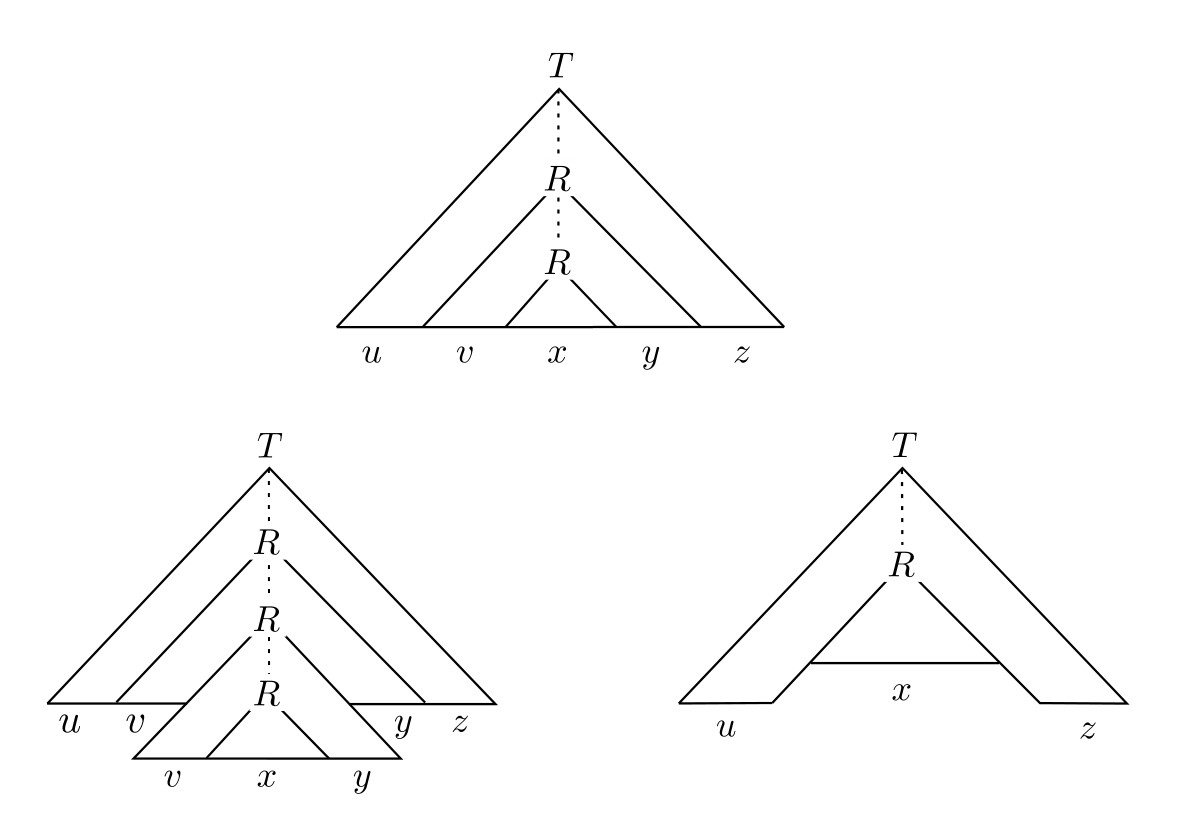
\includegraphics[scale=.5]{pumpLemmaCFG.jpg}
	\caption{Taken from the book}
\end{figure}
\begin{example}[Application of pumping lemma]
	Consider the language $\{a^nb^nc^n\mid n\geq 0\}$. Let $p\in \NN$, and consider the word $w = a^pb^pc^p$. Of course $w\in \Ll$ and $|w| \geq 0$. Any partitioning $w = uvxyz$ satisfying (1) - (2). By the structure of $w$, $|vxy|\leq p$ implies $vxy\in a^*b^* + b^*c^*$. Therefore, consider $i=2$, then
	$w_2 = uv^2xy^2z$ has more $a$ from $c$, or more $c$ than $a$, or more $b$ than $a,c$. Either way - $w_2\notin \Ll(\Gg)$.
\end{example}


